\section{Human-Robot Interaction}
\label{sec:hri}

\subsection{Graphics User Interface}
\label{subsec:gui}
As a domestic service robot, smooth GUI interaction is neccesary. 
One of the advantages of Pepper is that it has a laptop on its breast, which makes GUI possible. 
We designed a user-friendly and cross-platform interface so even people unfamiliar to robotics can quickly operate on Pepper. 

We have put twenty applications on the GUI so far, including Motion, Conversation, Vision, Joints, etc. 
In Motion, the operator can make the robot move a given distance to a given direction, or just move by a constant velocity.
In Conversation, the operator can chat with Pepper using English or Chinese.
In Vision, camera information is integrated. All images Pepper captured will be displayed here and the resolution is modifiable.
In Joints, all joints' status are listed for developer to debug.
We wish such GUI can help Pepper more powerful and useful.

\begin{figure}[!h]

    \centering
    \subfigure[Home page]{\label{fig11}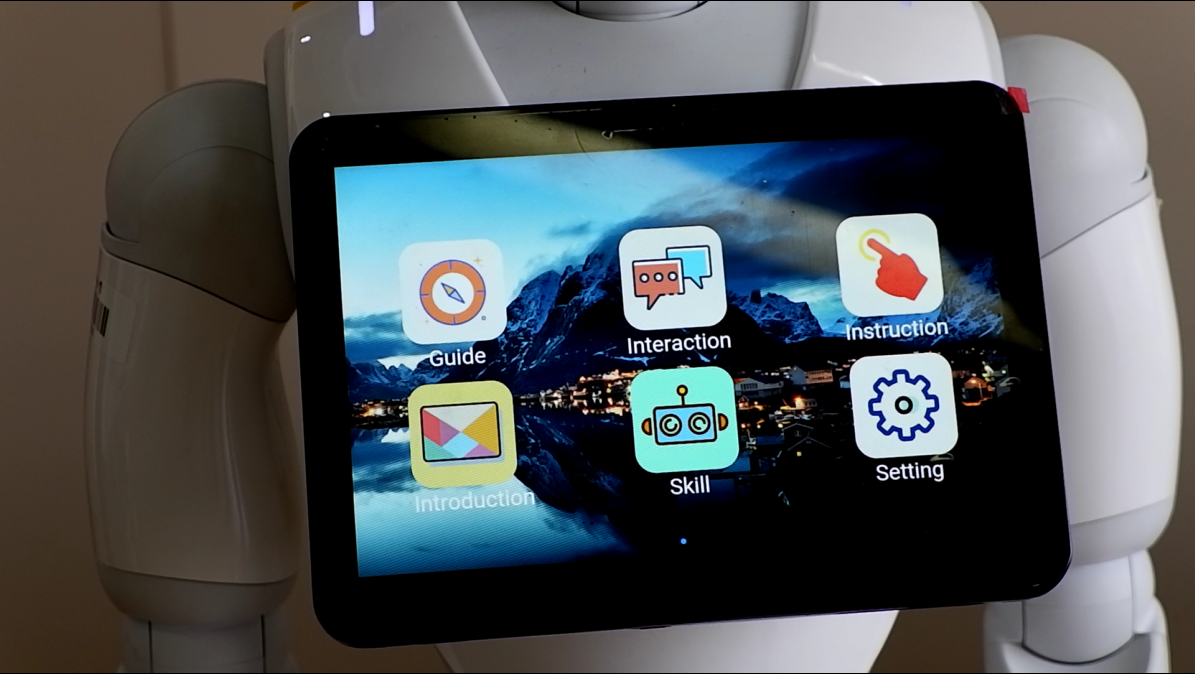
\includegraphics[width=2.5in]{figs/gui1_1.png}}
    \hspace{0.2in}
    \subfigure[Vision page]{\label{fig12}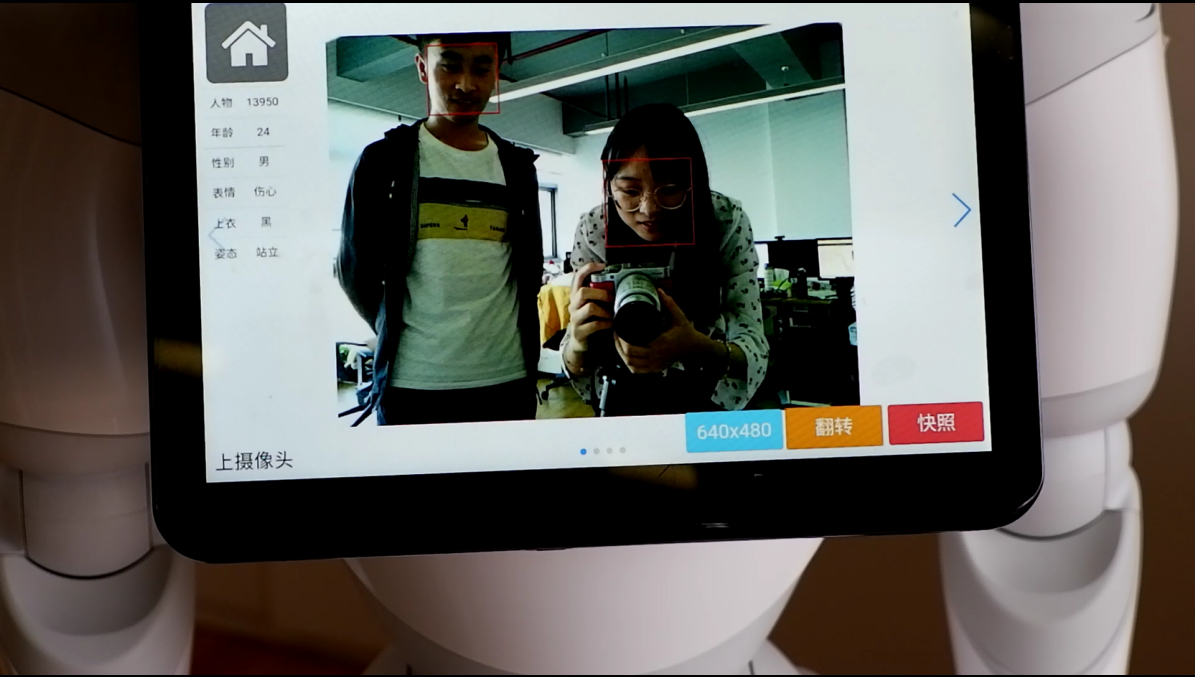
\includegraphics[width=2.5in]{figs/gui1_2.png}}\\
    
    \subfigure[Depth image page]{\label{fig13}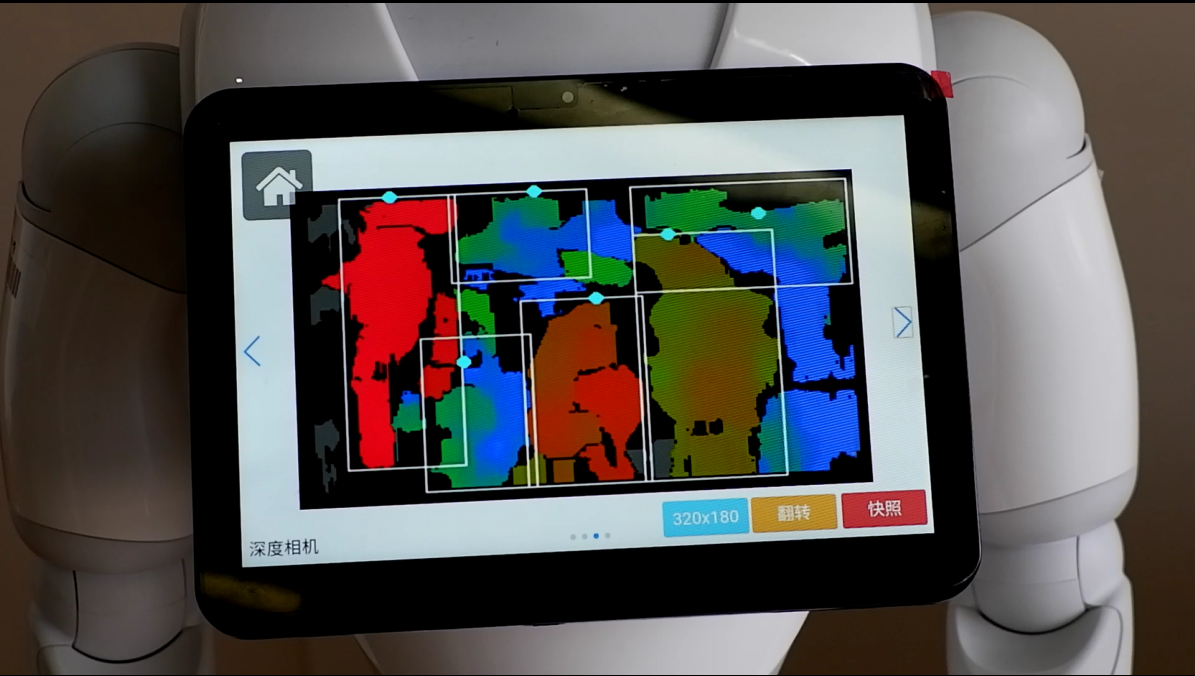
\includegraphics[width=2.5in]{figs/gui1_3.png}}
    \hspace{0.2in}
    \subfigure[Joints page]{\label{fig14}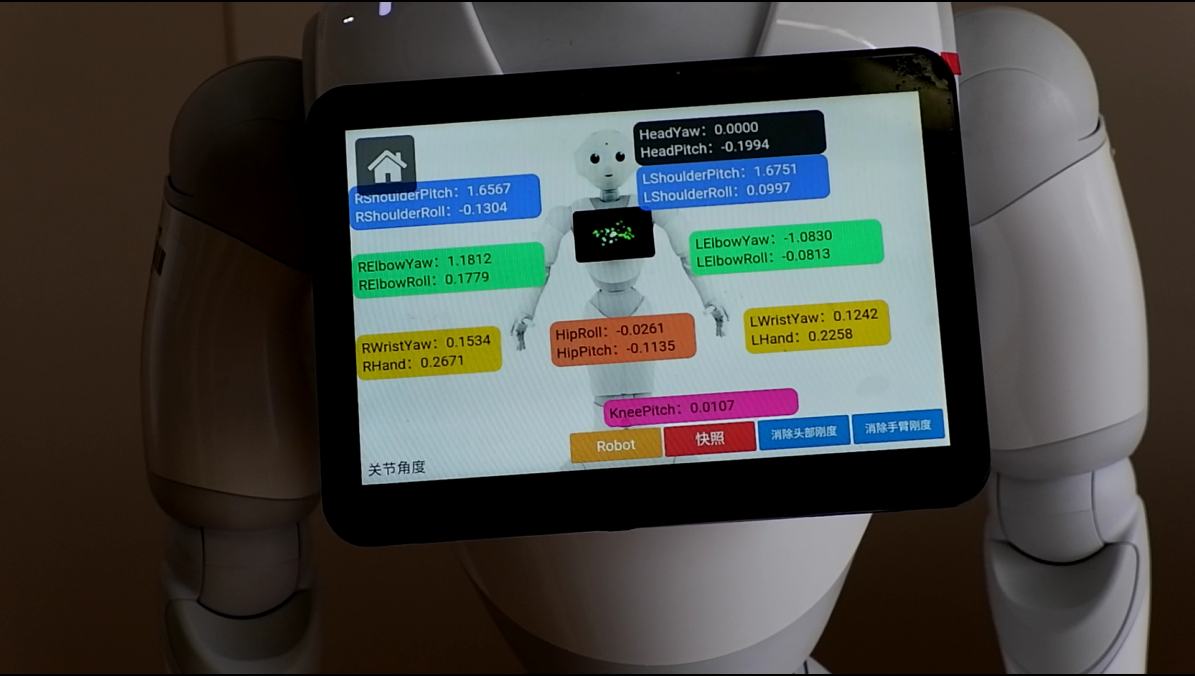
\includegraphics[width=2.5in]{figs/gui1_4.png}}

    \subfigure[Action teaching page]{\label{fig15}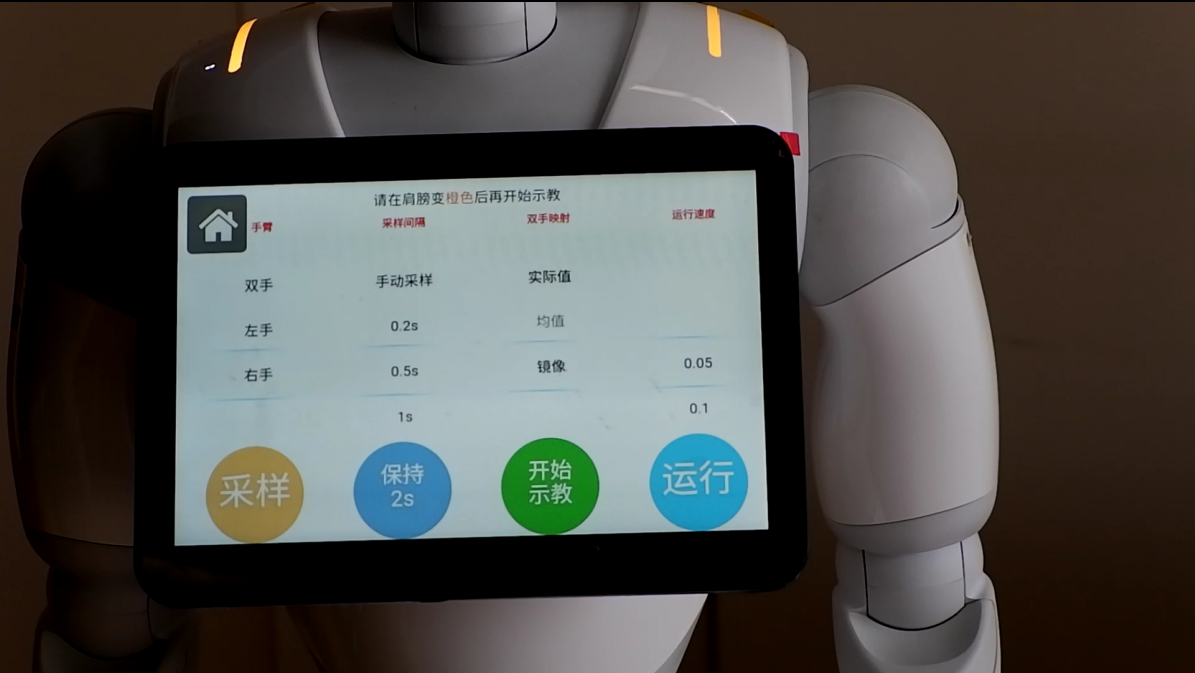
\includegraphics[width=2.5in]{figs/gui1_5.png}}
    \hspace{0.2in}
    \subfigure[Conversation page]{\label{fig16}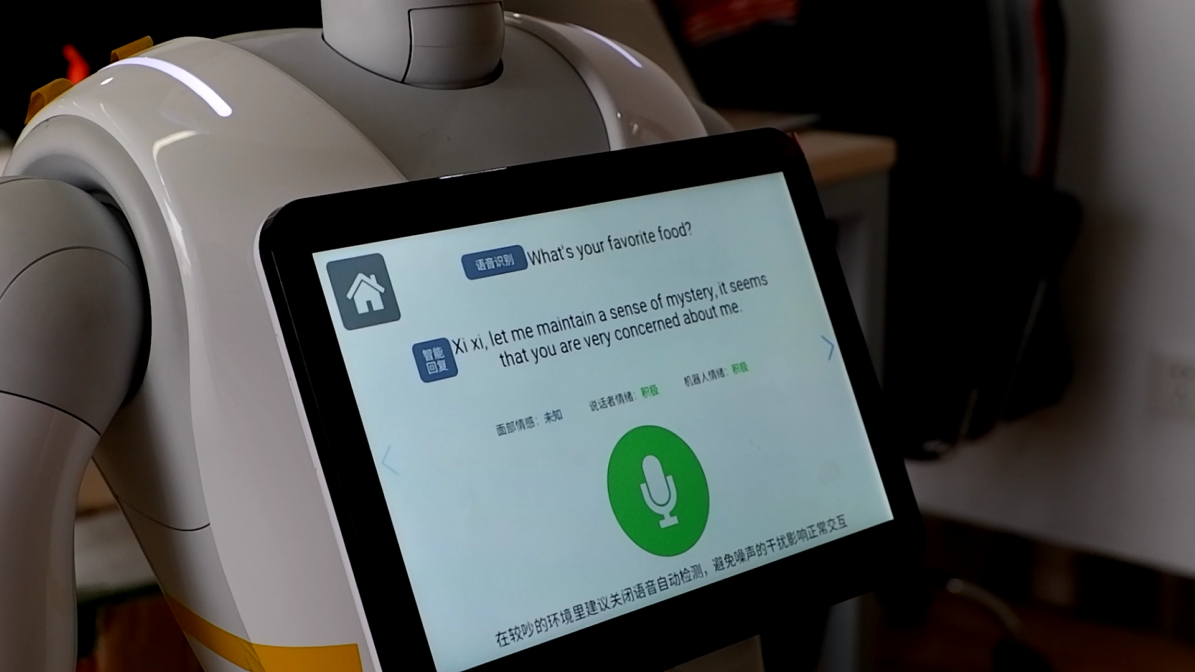
\includegraphics[width=2.5in]{figs/gui1_6.png}}


    \caption{GUI on Pepper's pad}
    
    \label{figb} %% label for entire figure
    
    \end{figure}

\subsection{Speech Interaction}
\label{subsec:speech}
As mentioned in \ref{subsec:gui}, we develop a conversation function. 
Language is an important interaction way in daily life.
As a domestic service robot, it should have the ability to understand natural language.
Our conversation applicaiton is powered by Xunfei cloud speech engine.
The demonstration video has been uploaded to https://www.youtube.com/channel/UCE5ceR\_uX-Hz3IIJx70lOrQ.
However, this function is triggered by pad touch, which makes the chat not so less smooth.
We are trying to make Pepper can detect and process speech of interest in real time.

\subsection{Touch Interaction}
\label{subsec:otherinteraction}
To make Pepper look smarter, we develop some other interaction ways to enrich its behaviors.
When someone touches its head, it would say something like "Huh, I feel a warm hand on my head".
And if Pepper's hand is being grabed, it will softly close hand and hold you, and greet you.
What's more, whenever pad or tactile sensors are touched, Pepper will look at that direction and speak or perform some body languages corresponding the condition.
Such touch interaction is funny and important.
It shows the robot is perceiving environment and ready to work.

For us developer, tactile sensors can do more.
There are three parallel tactile sensors on Pepper's head.
We designed a state machine to judge the touch direction.
If the touch is front to back, the head stiffness will be toggled.
If the touch is back to front, the arm stiffness will be toggled.
If the hand is touched more than 3 seconds, corresponding arm stiffness wil be toggled.
When we want to change some stiffness, we just need touch the robot rather than back to computer and run some codes.